\documentclass[11pt,letterpaper,boxed]{pset}

\usepackage[margin=0.75in]{geometry}
\usepackage{ulem}

\begin{document}

    \problemlist{PHYS051 HW09}
    \begin{center}
        *P34.9, SUP9.1, P36.3, P36.9, E36.44, E36.50
    \end{center}
    
    \begin{problem} [*P34.9]
        A rod with length $L$, mass $m$, and resistance $R$ slides without friction down parallel conducting rails of negligible resistance, as in Fig. 34-59. The rails are connected together at the bottom as shown, forming a conducting loop with the rod as the top member. The plane of the rails makes an angle $\theta$ with the horizontal, and a uniform magnetic field $\Vec{B}$ exists throughout the region. 
        
        \begin{enumerate}
            \item [a.] Show that the rod acquires a steady-state terminal velocity whose magnitude is
            \[v = \frac{mgR}{B^2L^2}\frac{\text{sin} \theta}{\text{cos}^2 \theta}.\]
            \item [b.] Show that the rate at which the internal energy of the rod is increasing is equal to the rate at which the rod is losing gravitational potential energy.
            \item [c.] Discuss the situation if $\Vec{B}$ were directed down instead of up.
        \end{enumerate}
    \end{problem}
    
    \begin{figure*} [ht]
        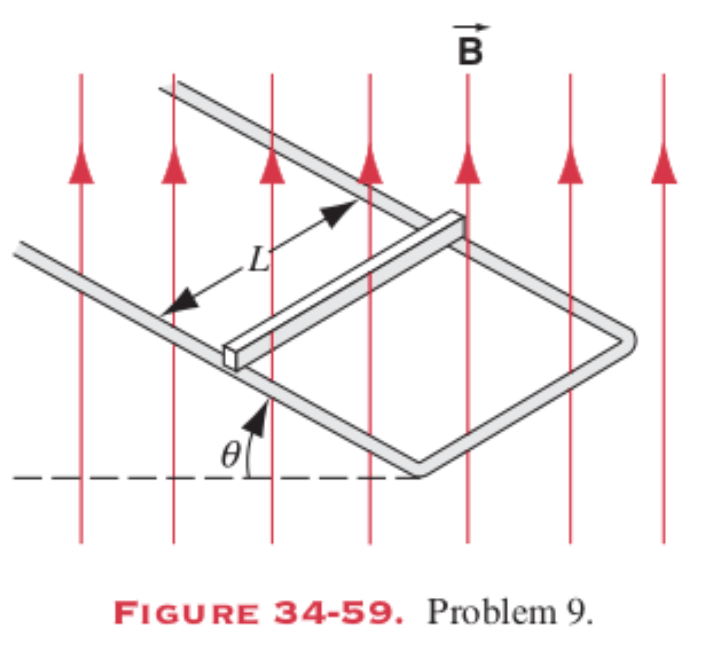
\includegraphics[width=125px]{HW9Images/P34-9.png}
        \label{fig:P34-9}
    \end{figure*}
    \newpage
    
    \begin{problem} [SUP9.1]
        The design of some electronic devices can involve circuit boards with broad conducting copper planes, in addition to the usual use of narrow wires. Two such adjacent planes can be a source of inadvertent inductance in a circuit. We will approximate this effect by considering two large, thin parallel conducting plates situated a distance $d$ apart, and carrying a current $I$ in parallel but opposite directions. Let the width $w$ and the length $h$ parallel to the direction of current flow be much larger than $d$, so that edge fringing effects may be neglected. (Let the plates have vanishingly small thickness.)
        
        \begin{enumerate}
            \item [a.] Determine the magnetic field $\Vec{B}$ everywhere due to this configuration of current.
            \item [b.] Use the method of flux linkage to find the effective inductance of the two plates.
            \item [c.] Verify the answer to part (b) by using the method of energy storage.
        \end{enumerate}
    \end{problem}
    
    \begin{figure*} [ht]
        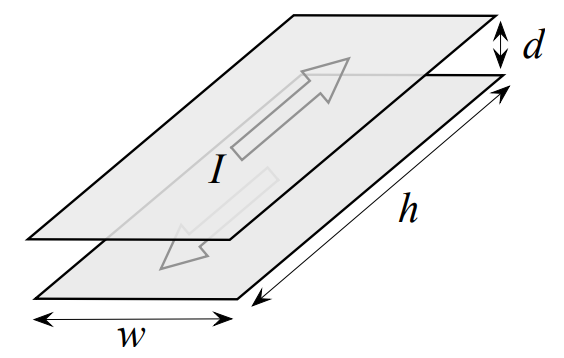
\includegraphics[width=125px]{HW9Images/SUP9-1.png}
        \label{fig:E34-23}
    \end{figure*}
    \newpage
    
    \begin{problem} [P36.3]
        Two long, parallel wires, each of radius $a$, whose centers are a distance $d$ apart carry equal currents in opposite directions. Show that, neglecting the flux within the wires themselves, the inductance of a length $l$ of such a pair of wires is given by 
        
        \[L = \frac{\mu_0l}{\pi} \text{ln}\frac{d-a}{a}.\]
        
        See Sample Problem 33-4. (Hint: Calculate the flux through a rectangle of which the wires form two opposite sides.)
    \end{problem}
    \newpage
    
    \begin{problem} [P36.9]
        \begin{enumerate}
            \item [a.] Find an expression for the energy density as a function of the radial distance $r$ for a toroid of rectangular cross section. 
            \item [b.] Integrating the energy density over the volume of the toroid, calculate the total energy stored in the field of the toroid. 
            \item [c.] Using Eq. 36-10, evaluate the energy stored in the toroid directly from the inductance and compare with (b).
        \end{enumerate}
        
        Pg. 825, Eq. 36-10 [\textit{Inductance of a Toroid}]: $L = \frac{N \Phi_B}{i} = \frac{\mu_0N^2h}{2\pi}\text{ln}\frac{b}{a}$
    \end{problem}
    \newpage
    
    \begin{problem} [E36.44]
        In the circuit shown in Fig. 36-22 the switch has been in position $a$ for a long time. It is now thrown to $b$. 
        
        \begin{enumerate}
            \item [a.] Calculate the frequency of the resulting oscillating current.
            \item [b.] What will be the amplitude of the current oscillations?
        \end{enumerate}
    \end{problem}
    
    \begin{figure*} [ht]
        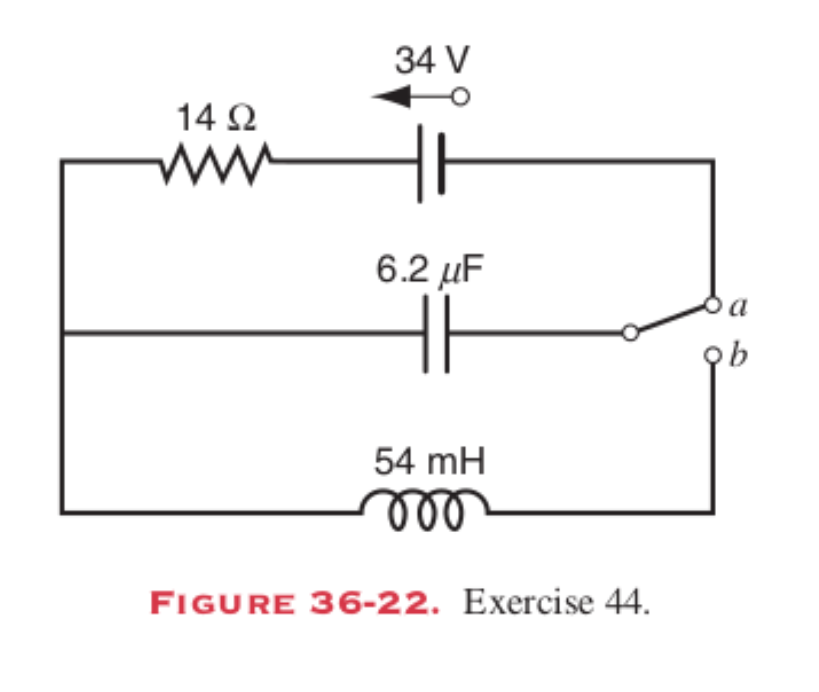
\includegraphics[width=125px]{HW9Images/E36-44.png}
        \label{fig:E36-44}
    \end{figure*}
    \newpage
    
    \begin{problem}[E36.50]
        In Fig. 36-23, the 900-$\mu$F capacitor is initially charged to 100 V and the 100-$\mu$F capacitor is uncharged. Describe in detail how one might charge the 100-$\mu$F capacitor to 300V by manipulating switches S$_1$ and S$_2$.
    \end{problem}
    
    \begin{figure*} [ht]
        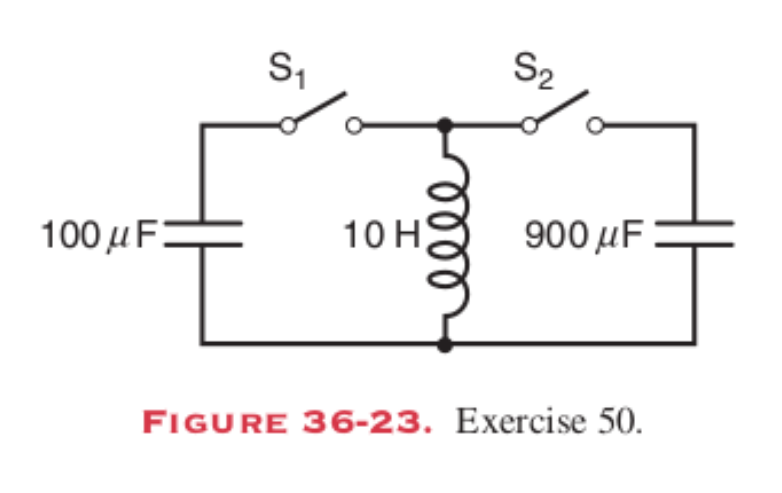
\includegraphics[width=125px]{HW9Images/E36-50.png}
        \label{fig:E36-50}
    \end{figure*}
\end{document}